\documentclass[12pt]{beamer}

\usepackage[brazil]{babel}
\usepackage[utf8]{inputenc}
\usepackage[T1]{fontenc}
\usepackage{animate}
\usepackage{amsbsy}
\usepackage{amsfonts}
\usepackage{amsmath}
\usepackage{amssymb}
\usepackage{amsthm}
\usepackage[toc,page,title,titletoc]{appendix}
\usepackage{dsfont}
\usepackage{esvect}
\usepackage[labelfont=bf]{caption}
\usepackage{subcaption}
\usepackage{float}
\usepackage[Glenn]{fncychap}%Sonny %Conny %Lenny %Glenn %Renje %Bjarne %Bjornstrup
\usepackage{graphicx}
\usepackage{indentfirst}%Para indentar os paragrafos automaticamente
\usepackage{lipsum}
\usepackage{longtable}
\usepackage{mathtools}
\usepackage{listings}%Inserir codigo do R no latex
\usepackage{multirow}
\usepackage{multicol}
\usepackage{csquotes}
\usepackage[style=authoryear,
			%style = bwl-FU,
			maxcitenames = 2,
			terseinits = true,
			natbib = true, 
			maxbibnames = 99]{biblatex}
\addbibresource{Referencias/Referencias.bib}
\usepackage[figuresright]{rotating}
\usepackage{spalign}
\usepackage{pgfplots}
\pgfplotsset{compat=1.17}
\usepackage{tikz}
\usepackage{color, colortbl}
\usepackage{url}
\usepackage{ragged2e}%para justificar o texto dentro de algum ambiente
\definecolor{Gray}{gray}{0.9}
\definecolor{LightCyan}{rgb}{0.88,1,1}


\usepackage[all]{xy}
\usepackage{hyperref,bookmark}
\hypersetup{
  colorlinks=true,
  linkcolor=blue,
  citecolor=red,
  filecolor=blue,
  urlcolor=blue,
}

\usetheme{Madrid}
\usecolortheme[RGB={193,0,0}]{structure}

%\setbeamertemplate{footline}[frame number]
%\setbeamertemplate{footline}[text line]{%
%  \parbox{\linewidth}{\vspace*{-8pt}\hfill\date{}\hfill\insertshortauthor\hfill\insertpagenumber}}
\beamertemplatenavigationsymbolsempty
\renewcommand{\vec}[1]{\mbox{\boldmath$#1$}}
\newtheorem{Teorema}{Teorema}
\newtheorem{Proposicao}{Proposição}
\newtheorem{Definicao}{Definição}
\newtheorem{Corolario}{Corolário}
\newtheorem{Demonstracao}{Demonstração}
\newcommand{\bx}{\ensuremath{\bar{x}}}
\newcommand{\Ho}{\ensuremath{H_{0}}}
\newcommand{\Hi}{\ensuremath{H_{1}}}


\apptocmd{\frame}{}{\justifying}{} % Allow optional arguments after frame.

\title{Iniciação à Estatística}
\author{Prof. Fernando de Souza Bastos\texorpdfstring{\\ fernando.bastos@ufv.br}{}}
\institute{Departamento de Estatística\texorpdfstring{\\ Universidade Federal de Viçosa}{}\texorpdfstring{\\ Campus UFV - Viçosa}{}}
\date{}
\newcommand\mytext{Aula 1}
\newcommand\mytextt{Fernando de Souza Bastos}
\newcommand\mytexttt{\url{https://ufvest.github.io/}}

\makeatletter
\setbeamertemplate{footline}
{
  \leavevmode%
  \hbox{%
  \begin{beamercolorbox}[wd=.3\paperwidth,ht=2.25ex,dp=1ex,center]{author in head/foot}%
    \usebeamerfont{author in head/foot}\mytext
  \end{beamercolorbox}%
  \begin{beamercolorbox}[wd=.3\paperwidth,ht=2.25ex,dp=1ex,center]{title in head/foot}%
    \usebeamerfont{title in head/foot}\mytextt
  \end{beamercolorbox}%
  \begin{beamercolorbox}[wd=.35\paperwidth,ht=2.25ex,dp=1ex,right]{site in head/foot}%
    \usebeamerfont{site in head/foot}\mytexttt\hspace*{2em}
    \insertframenumber{} / \inserttotalframenumber\hspace*{2ex} 
  \end{beamercolorbox}}%
  \vskip0pt%
}
\makeatother

\providecommand{\arcsin}{} \renewcommand{\arcsin}{\hspace{2pt}\textrm{arcsen}}
\providecommand{\sin}{} \renewcommand{\sin}{\hspace{2pt}\textrm{sen}}
%\newtheorem{Teorema}{Teorema}
%\newtheorem{Proposicao}{Proposição}
%\newtheorem{Definicao}{Definição}
%\newtheorem{Corolario}{Corolário}
%\newtheorem{Demonstracao}{Demonstração}

\titlegraphic{\hspace*{8cm}\href{https://fsbmat-ufv.github.io/}{
\includegraphics[width=2cm]{figs/mylogo.png}}
}

% Layout da pagina
\hypersetup{pdfpagelayout=SinglePage}
\begin{document}
%\SweaveOpts{concordance=TRUE}

\frame{\titlepage}

\begin{frame}{}
\frametitle{\bf Sumário}
\tableofcontents
\end{frame}

\section{Introdução}
\begin{frame}{}
	\frametitle{}
	\begin{block}{}
		\justifying
		\textit{``Você já parou para pensar em como os dados moldam a nossa realidade? Em cada etapa do seu trabalho ou estudo, em algum momento você vai se deparar com a necessidade de entender e interpretar dados. Seja na comparação de resultados, na confirmação de uma hipótese ou no desenvolvimento de uma nova ideia, os dados estarão sempre presentes, e saber como trabalhá-los será sua ferramenta mais poderosa.''}
	\end{block}
\end{frame}

\begin{frame}{}
	\frametitle{}
	\begin{block}{}
		\justifying
		\begin{center}
			\Large{\bf{Dados: Não dá para fugir deles!}}
		\end{center}
	\end{block}
\end{frame}

\begin{frame}{}
	\frametitle{}
	\begin{block}{}
		\justifying
		\begin{figure}[H]
			\centering
			\caption{Vivemos na Era do Big Data}
			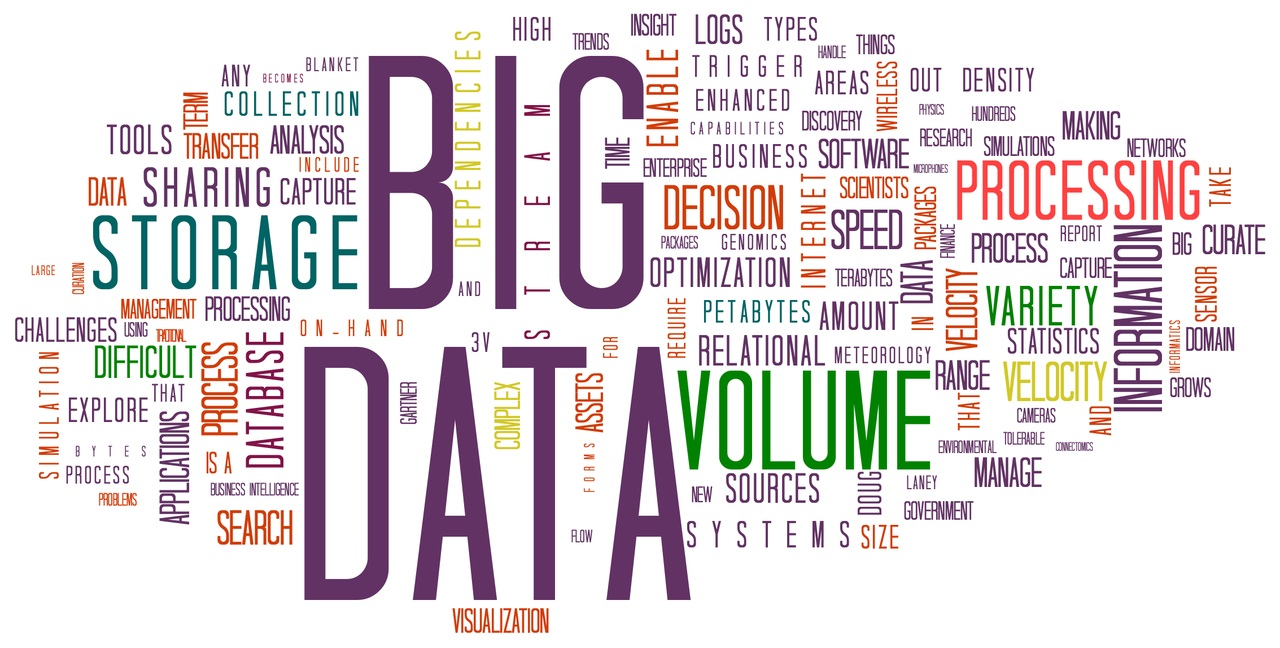
\includegraphics[scale=0.2]{figs/BigData.jpg}
			\subcaption*{\textbf{Fonte:} Revista Exame 2017 \citet{exame17}}
		\end{figure}
		\textit{``Imagine que, a cada segundo, milhares de dados são gerados no mundo inteiro. Vamos explorar esse universo de informações e aprender a tirar o melhor proveito dele!''}
	\end{block}
\end{frame}

\begin{frame}{}
	\frametitle{}
	\begin{block}{}
		\justifying
		\textbf{Alguns números impressionantes para vocês pensarem:}
		\begin{itemize}
			\item Google: mais de 5,5 bilhões de buscas por dia \cite{ardorseo}.\pause
			\item \citet{youtube}: mais de 2 bilhões de usuários e mais de 1 bilhão de horas de vídeos assistidos por dia.\pause
			\item Facebook: picos de 2,8 bilhões de usuários ativos diariamente \cite{internetstats}.\pause
			\item Instagram: Mais de 500 milhões de usuários diários utilizando o \textit{stories} \cite{InstagramStats}.\pause
			\item WhatsApp: mais de 100 bilhões de mensagens trocadas todos os dias \cite{WhatsappStats}.\pause
			\item Twitter: 500 milhões de tweets por dia \cite{TwitterStats}.
		\end{itemize}
		\textit{``A era digital está aqui, e cada clique seu gera um dado. Vamos aprender a navegar por esse oceano de informações?''}
	\end{block}
\end{frame}

\begin{frame}{}
	\frametitle{}
	\begin{block}{}
		\justifying
		\begin{itemize}
			\item Mais de 1,8 bilhões de sites e 4,6 bilhões de pessoas conectadas \cite{internetstats2}.\pause
			\item 5,7 bilhões de celulares ativos no mundo \cite{datareportal}.\pause
			\item Em 2030, teremos 50 bilhões de dispositivos conectados \cite{statista}.\pause
			\item Em 2025, a quantidade de dados gerados diariamente chegará a 463 exabytes \cite{seedscientific}.
		\end{itemize}
		\textit{``Esses números podem parecer assustadores, mas a Estatística vai te ajudar a colocar ordem nesse caos de dados!''}
	\end{block}
\end{frame}


\begin{frame}{}
	\frametitle{Introdução}
	\begin{block}{}
		\justifying
		\textbf{Estatística: Uma ferramenta poderosa!} A estatística nos permite tomar decisões inteligentes com base em dados. Com ela, você pode solucionar problemas de forma fundamentada e objetiva. Vamos explorar como ela pode ser aplicada em diversas situações do nosso dia a dia.
	\end{block}
\end{frame}

\begin{frame}{}
	\frametitle{Introdução}
	\begin{block}{}
		\justifying
		\textit{``A estatística é a arte de torturar os números até que eles confessem!''}\\
		*Como mentir com estatísticas \cite{huff2016mentir} (reedição de 1954)
		\begin{itemize}
			\item \textbf{Curiosidade:} A estatística pode ser usada para contar a verdade... ou para enganar! Vamos aprender como usá-la da maneira correta.
		\end{itemize}
	\end{block}
\end{frame}

\begin{frame}{}
	\frametitle{Introdução}
	\begin{block}{}
		\justifying
		Na primeira parte deste curso, nosso objetivo será:
		\begin{itemize}
			\item Organizar e interpretar dados de forma eficiente!
			\item Limpar e resumir os dados para facilitar a análise!
		\end{itemize}
		\pause
		\textbf{Essa é a base da Análise Exploratória de Dados (AED)}, onde vamos descobrir padrões e informações importantes escondidas nos números.
	\end{block}
\end{frame}

\begin{frame}{}
	\frametitle{Introdução}
	\begin{block}{}
		\justifying
		Vamos aprender a calcular medidas de posição e variabilidade, e também usar técnicas gráficas para entender melhor os dados. Essa é a etapa inicial para a construção de modelos e inferências estatísticas!
	\end{block}
\end{frame}

\begin{frame}{}
	\frametitle{Referências do Curso:}
	\begin{block}{}
		\justifying
		Vamos utilizar:
		\begin{itemize}
			\item \citetitle{roteiro}.
			\item (Sugestão de Livro) \citetitle{morettin2017estatistica} dos autores Wilton de Oliveira Bussab e Pedro Alberto Morettin;
			\item (Sugestão de Livro) 
			\citetitle{eric} dos autores Eric Batista Ferreira e Marcelo Silva de Oliveira.
		\end{itemize}
	\end{block}
\end{frame}


\begin{frame}[allowframebreaks]
\frametitle{\bf Referências}
\justifying
\printbibliography[heading=none]
\end{frame}


\end{document}
